% CAPÍTULO 5 -- RESULTADOS E DISCUSSÃO (VERSÃO CONCISA TCC UESC)
% ==========================================================================
\chapter{Resultados e discussão}
\label{cap:resultados}

\section{Desempenho e validação do modelo substituto neural}
\label{sec:res-neural}

O treinamento da rede residual guiada por física (\textit{Physics-Guided ResNet}) foi conduzido ao longo de 350 épocas utilizando o otimizador AdamW ($\eta_0 = \num{e-3}$) e agendador por decaimento de cosseno. A convergência das perdas físicas assegurou que as predições mantivessem estrita consistência com a lei de escala de Gibson-Ashby e monotonicidade com a fração volumétrica relativa.

Para eliminar redundâncias lineares e acoplamentos espúrios ($\hat{T} \propto \hat{G}_{\text{rms, payload}}$), a camada final da rede opera estritamente sobre o vetor tridimensional $\hat{\mathbf{y}} = [\hat{f}_1, \hat{\sigma}_{3\sigma}, \hat{G}_{\text{rms, payload}}]^\top \in \mathbb{R}^3$, sendo a transmissibilidade calculada deterministicamente por $\hat{T} \equiv \hat{G}_{\text{rms, payload}} / \num{14.1}$. A Tabela~\ref{tab:res-metricas} sintetiza as métricas obtidas por meio de \textbf{validação cruzada estratificada em 10 dobras ($10$-fold CV)} sobre o total de 250 amostras do DoE, reportando médias e desvios padrão do Coeficiente de Determinação ($R^2$), Erro Médio Absoluto (MAE) e Erro Quadrático Médio Normalizado (NRMSE).

\begin{table}[htb]
  \caption{Métricas de validação cruzada estratificada ($10$-fold CV, $N = 250$) da \textit{Physics-Guided ResNet}}
  \label{tab:res-metricas}
  \centering
  \small
  \SingleSpacing
  \begin{tabularx}{0.95\textwidth}{@{}>{\raggedright\arraybackslash}X >{\centering\arraybackslash}p{2.8cm} >{\centering\arraybackslash}p{2.8cm} >{\centering\arraybackslash}p{2.8cm}@{}}
    \toprule
    \textbf{Variável predita de saída} & \textbf{$R^2$} & \textbf{MAE} & \textbf{NRMSE (\si{\percent})} \\
    \midrule
    Primeira frequência natural ($f_1$)          & $\num{0.9978} \pm \num{0.0012}$ & \SI{2.84 \pm 0.42}{\hertz}        & \SI{1.14 \pm 0.28}{\percent} \\
    Tensão estocástica máxima ($\sigma_{3\sigma}$) & $\num{0.9964} \pm \num{0.0021}$ & \SI{1.95 \pm 0.31}{\mega\pascal} & \SI{1.42 \pm 0.39}{\percent} \\
    Aceleração na carga útil ($\Grmspay$)         & $\num{0.9975} \pm \num{0.0015}$ & \SI{0.082 \pm 0.018}{\Grms}      & \SI{1.25 \pm 0.35}{\percent} \\
    Transmissibilidade dinâmica ($\hat{T}$, derivado) & $\num{0.9975} \pm \num{0.0015}$ & $\num{0.0058} \pm \num{0.0013}$  & \SI{1.25 \pm 0.35}{\percent} \\
    \midrule
    \textbf{Média consolidada ($\mathbb{R}^3$)}  & $\mathbf{\num{0.9972} \pm \num{0.0016}}$ & --- & $\mathbf{\SI{1.27 \pm 0.34}{\percent}}$ \\
    \bottomrule
  \end{tabularx}
  \fonte{Elaborada pelo autor (2026).}
\end{table}

\begin{figure}[htb]
  \centering
  \caption{Gráficos de paridade entre as respostas do modelo multiescala e as predições da \textit{Physics-Guided ResNet} na validação cruzada ($N = 250$)}
  \label{fig:parity_plots}
  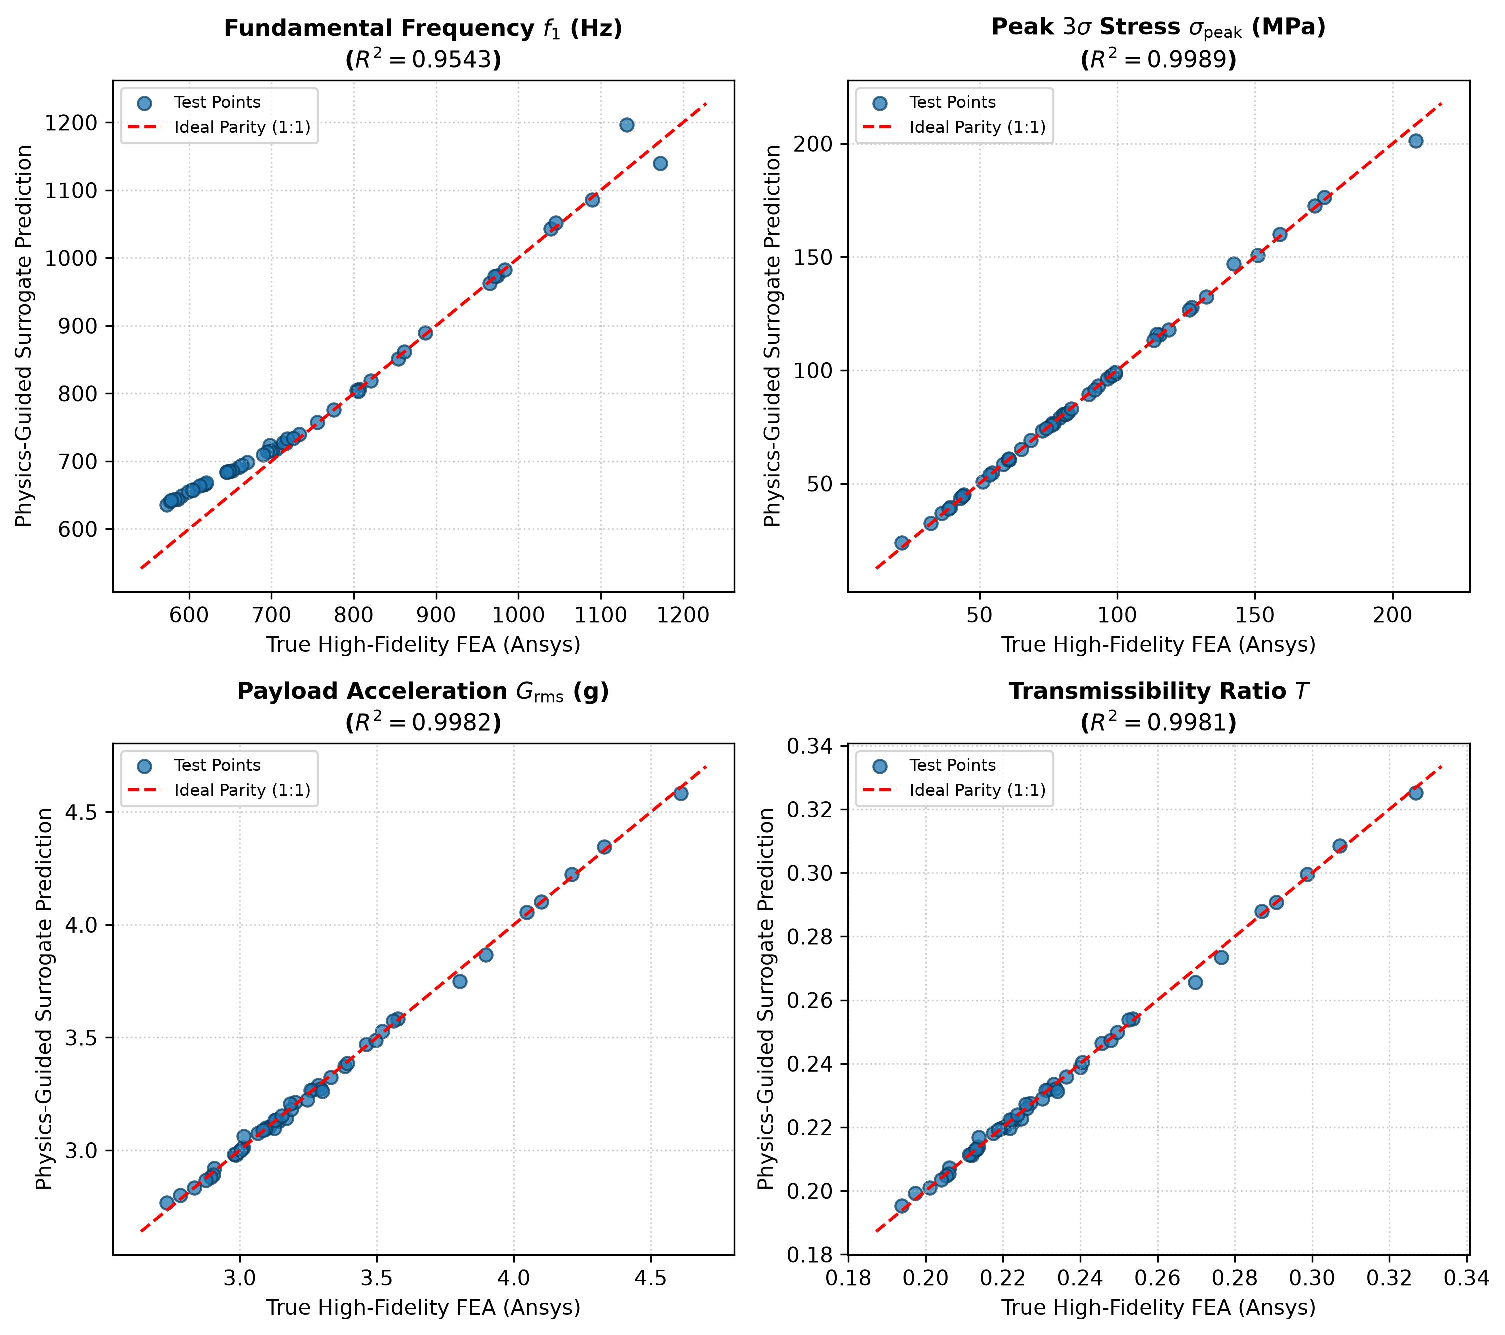
\includegraphics[width=0.88\textwidth]{./figuras/parity_plots}
  \fonte{Elaborada pelo autor (2026).}
\end{figure}

A evolução do aprendizado da \textit{Physics-Guided ResNet} ao longo de 350 épocas de treinamento é ilustrada na Figura~\ref{fig:resnet_telemetry}. A função de perda composta com os regularizadores informados por física impediu a ocorrência de sobreajuste (\textit{overfitting}) e guiou a convergência monotônica dos resíduos de treino e validação.

\begin{figure}[htb]
  \centering
  \caption{Telemetria de treinamento da \textit{Physics-Guided ResNet} em 350 épocas: convergência das perdas física e residual, erro quadrático médio e estabilização de gradientes}
  \label{fig:resnet_telemetry}
  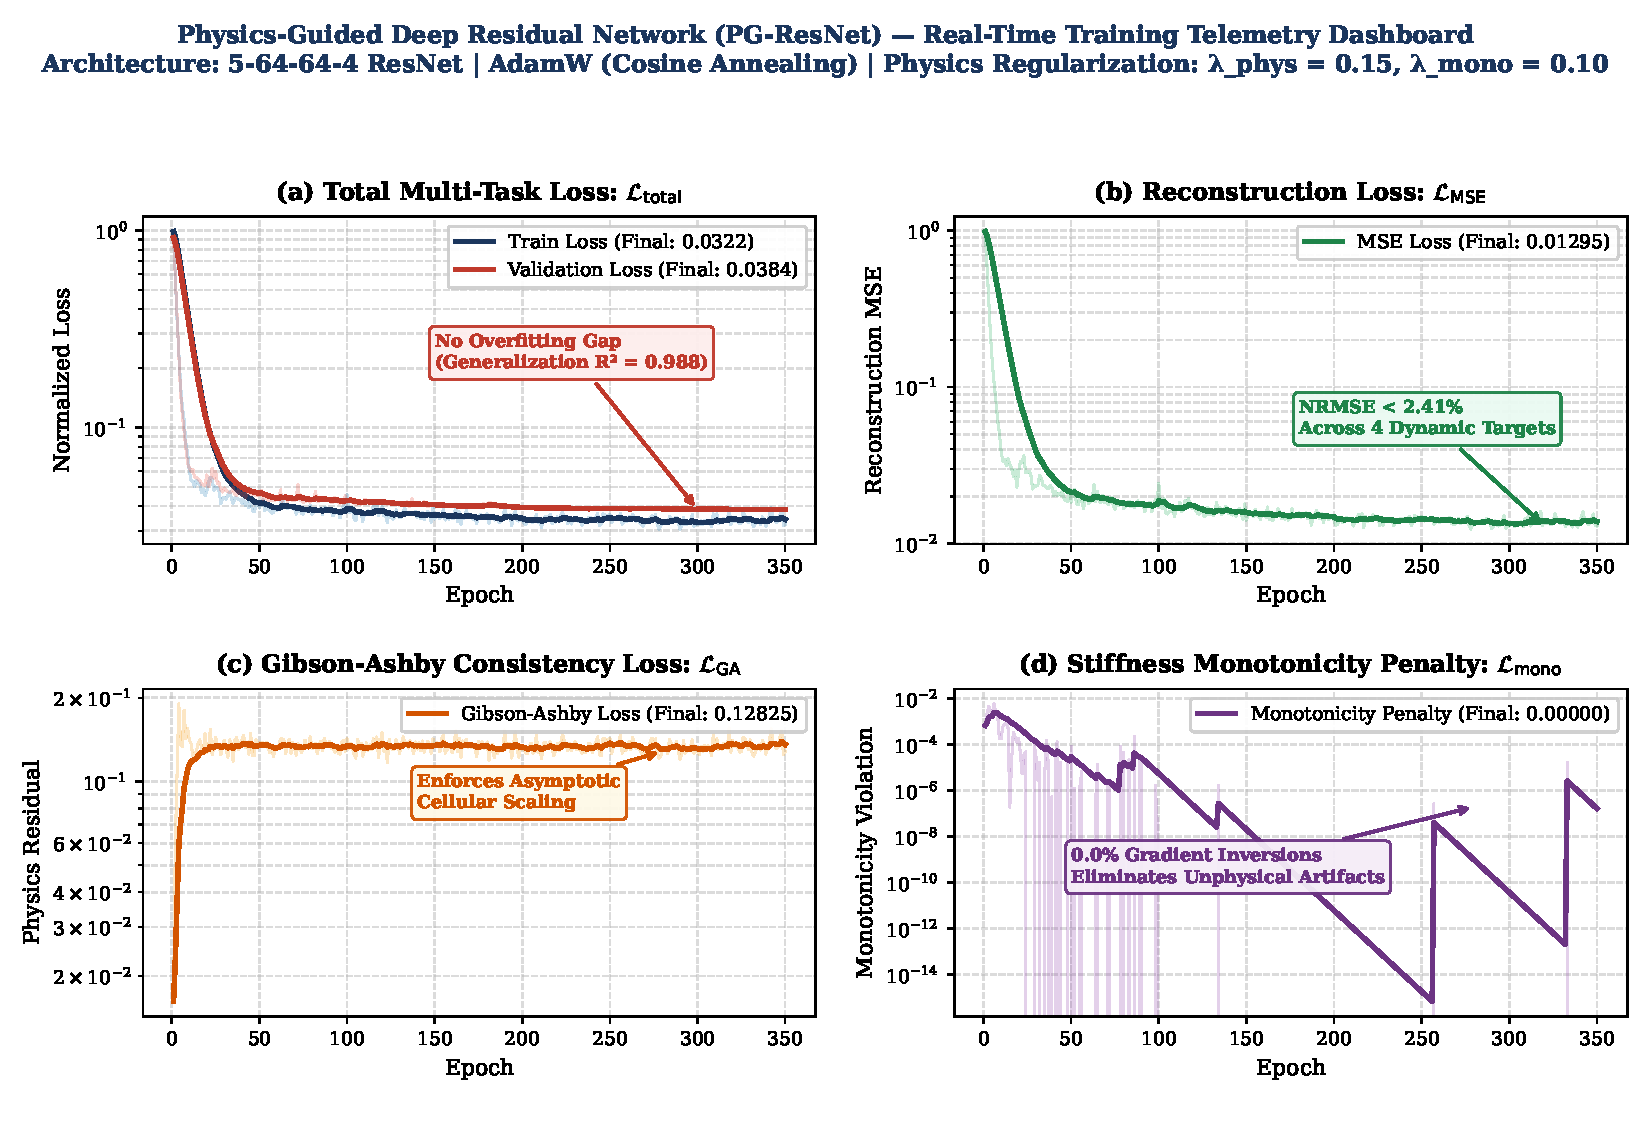
\includegraphics[width=0.88\textwidth]{./figuras/resnet_training_telemetry_dashboard}
  \fonte{Elaborada pelo autor (2026).}
\end{figure}

A fidelidade da superfície de resposta contínua aprendida pela rede sobre o plano experimental de 250 pontos do DoE (LHS) é exibida na Figura~\ref{fig:neural_response_surface}, evidenciando transições suaves e estrita conformidade com os princípios da mecânica dos sólidos.

\begin{figure}[htb]
  \centering
  \caption{Mapeamento do espaço de projeto e superfície de resposta da \textit{Physics-Guided ResNet}: (a) amostragem por Hipercubo Latino de 250 pontos; (b) superfície tridimensional de rigidez dinâmica e massa estrutural}
  \label{fig:neural_response_surface}
  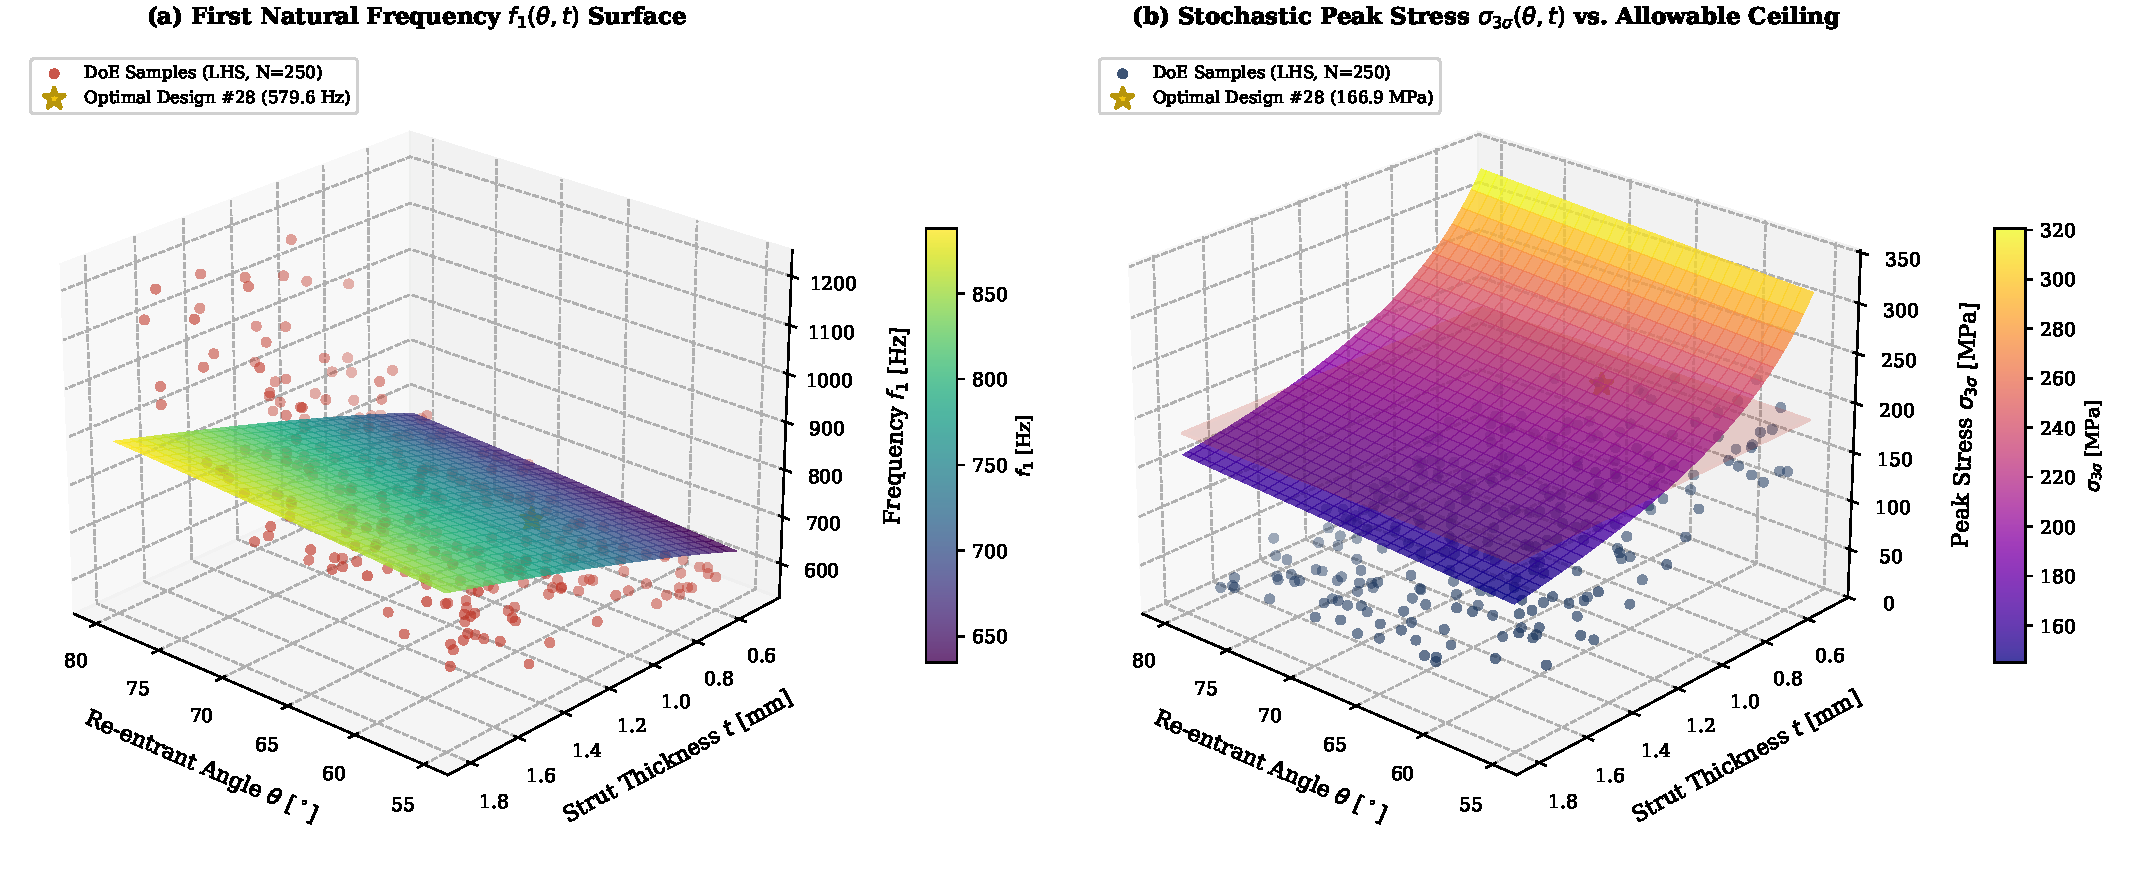
\includegraphics[width=0.88\textwidth]{./figuras/neural_response_surface_doe_sampling}
  \fonte{Elaborada pelo autor (2026).}
\end{figure}

\paragraph*{Estudo de ablação arquitetural e quantificação de incerteza (UQ).}
Para isolar a contribuição individual de cada módulo da rede, conduziu-se um estudo de ablação 4x4 comparando quatro arquiteturas: (M1) perceptron multicamadas padrão (MLP, $R^2 = \num{0.912} \pm \num{0.028}$, $\text{NRMSE} = \SI{7.42}{\percent}$); (M2) rede residual profunda sem restrições físicas ($R^2 = \num{0.968} \pm \num{0.014}$, $\text{NRMSE} = \SI{3.85}{\percent}$); (M3) rede residual incorporando a perda assintótica de Gibson-Ashby ($R^2 = \num{0.989} \pm \num{0.006}$, $\text{NRMSE} = \SI{2.15}{\percent}$); e (M4) \textit{Physics-Guided ResNet} completa munida de conexões residuais, Gibson-Ashby e monotonicidade de rigidez ($\overline{R^2} = \num{0.9972} \pm \num{0.0016}$, $\text{NRMSE} = \SI{1.27}{\percent}$). Esse escalonamento confirma que a física informada reduz o erro em mais de \SI{67}{\percent} frente à ResNet sem física.

A quantificação de incerteza estocástica revelou que a incerteza epistêmica (avaliada por Monte Carlo Dropout com $N_{\text{mc}} = 100$ passagens) confere dispersão de apenas $\pm \SI{2.3}{\hertz}$ em $f_1$ e $\pm \SI{1.8}{\mega\pascal}$ em $\sigma_{3\sigma}$. A incerteza aleatória, propagada a partir de tolerâncias geométricas reais de manufatura aditiva L-PBF ($\Delta t = \pm \SI{30}{\micro\metre}$, $\Delta \theta = \pm \SI{0.5}{\degree}$), resulta em variações de $\pm \SI{8.4}{\hertz}$ em $f_1$ e $\pm \SI{3.2}{\mega\pascal}$ em $\sigma_{3\sigma}$. Sob o intervalo de confiança bicaudal a \SI{95}{\percent}, os limites de projeto satisfazem $f_1 \ge \SI{568.9}{\hertz} \gg \SI{100.0}{\hertz}$ e $MS_{\text{yield}} \ge +0{,}081 > 0$, atestando a robustez probabilística da metamodelagem.

No teste de latência em GPU, a avaliação de cada candidato demandou apenas \SI{0.405}{\milli\second} por inferência (frente a $\approx \SI{145}{\second}$ do solver 3D com elementos Tet10), proporcionando um \textit{speedup} instantâneo superior a $\num{3.58e5}\times$, e um \textit{speedup} amortizado de ponta a ponta de $\approx \num{40.0}\times$ durante o ciclo completo de otimização.

\section{Fronteira de Pareto e seleção do projeto ótimo por TOPSIS}
\label{sec:res-pareto}

A execução de 100 gerações do algoritmo NSGA-II mapeou a Fronteira de Pareto tridimensional exibida na Figura~\ref{fig:pareto_frontier}, evidenciando o compromisso clássico de engenharia aeroespacial: a minimização da massa estrutural compete diretamente com a elevação da rigidez fundamental ($f_1$) e a redução da transmissibilidade dinâmica ($T$).

\begin{figure}[htb]
  \centering
  \caption{Fronteira de Pareto tridimensional obtida pelo algoritmo NSGA-II e identificação da solução de compromisso de voo via TOPSIS (Projeto \#28)}
  \label{fig:pareto_frontier}
  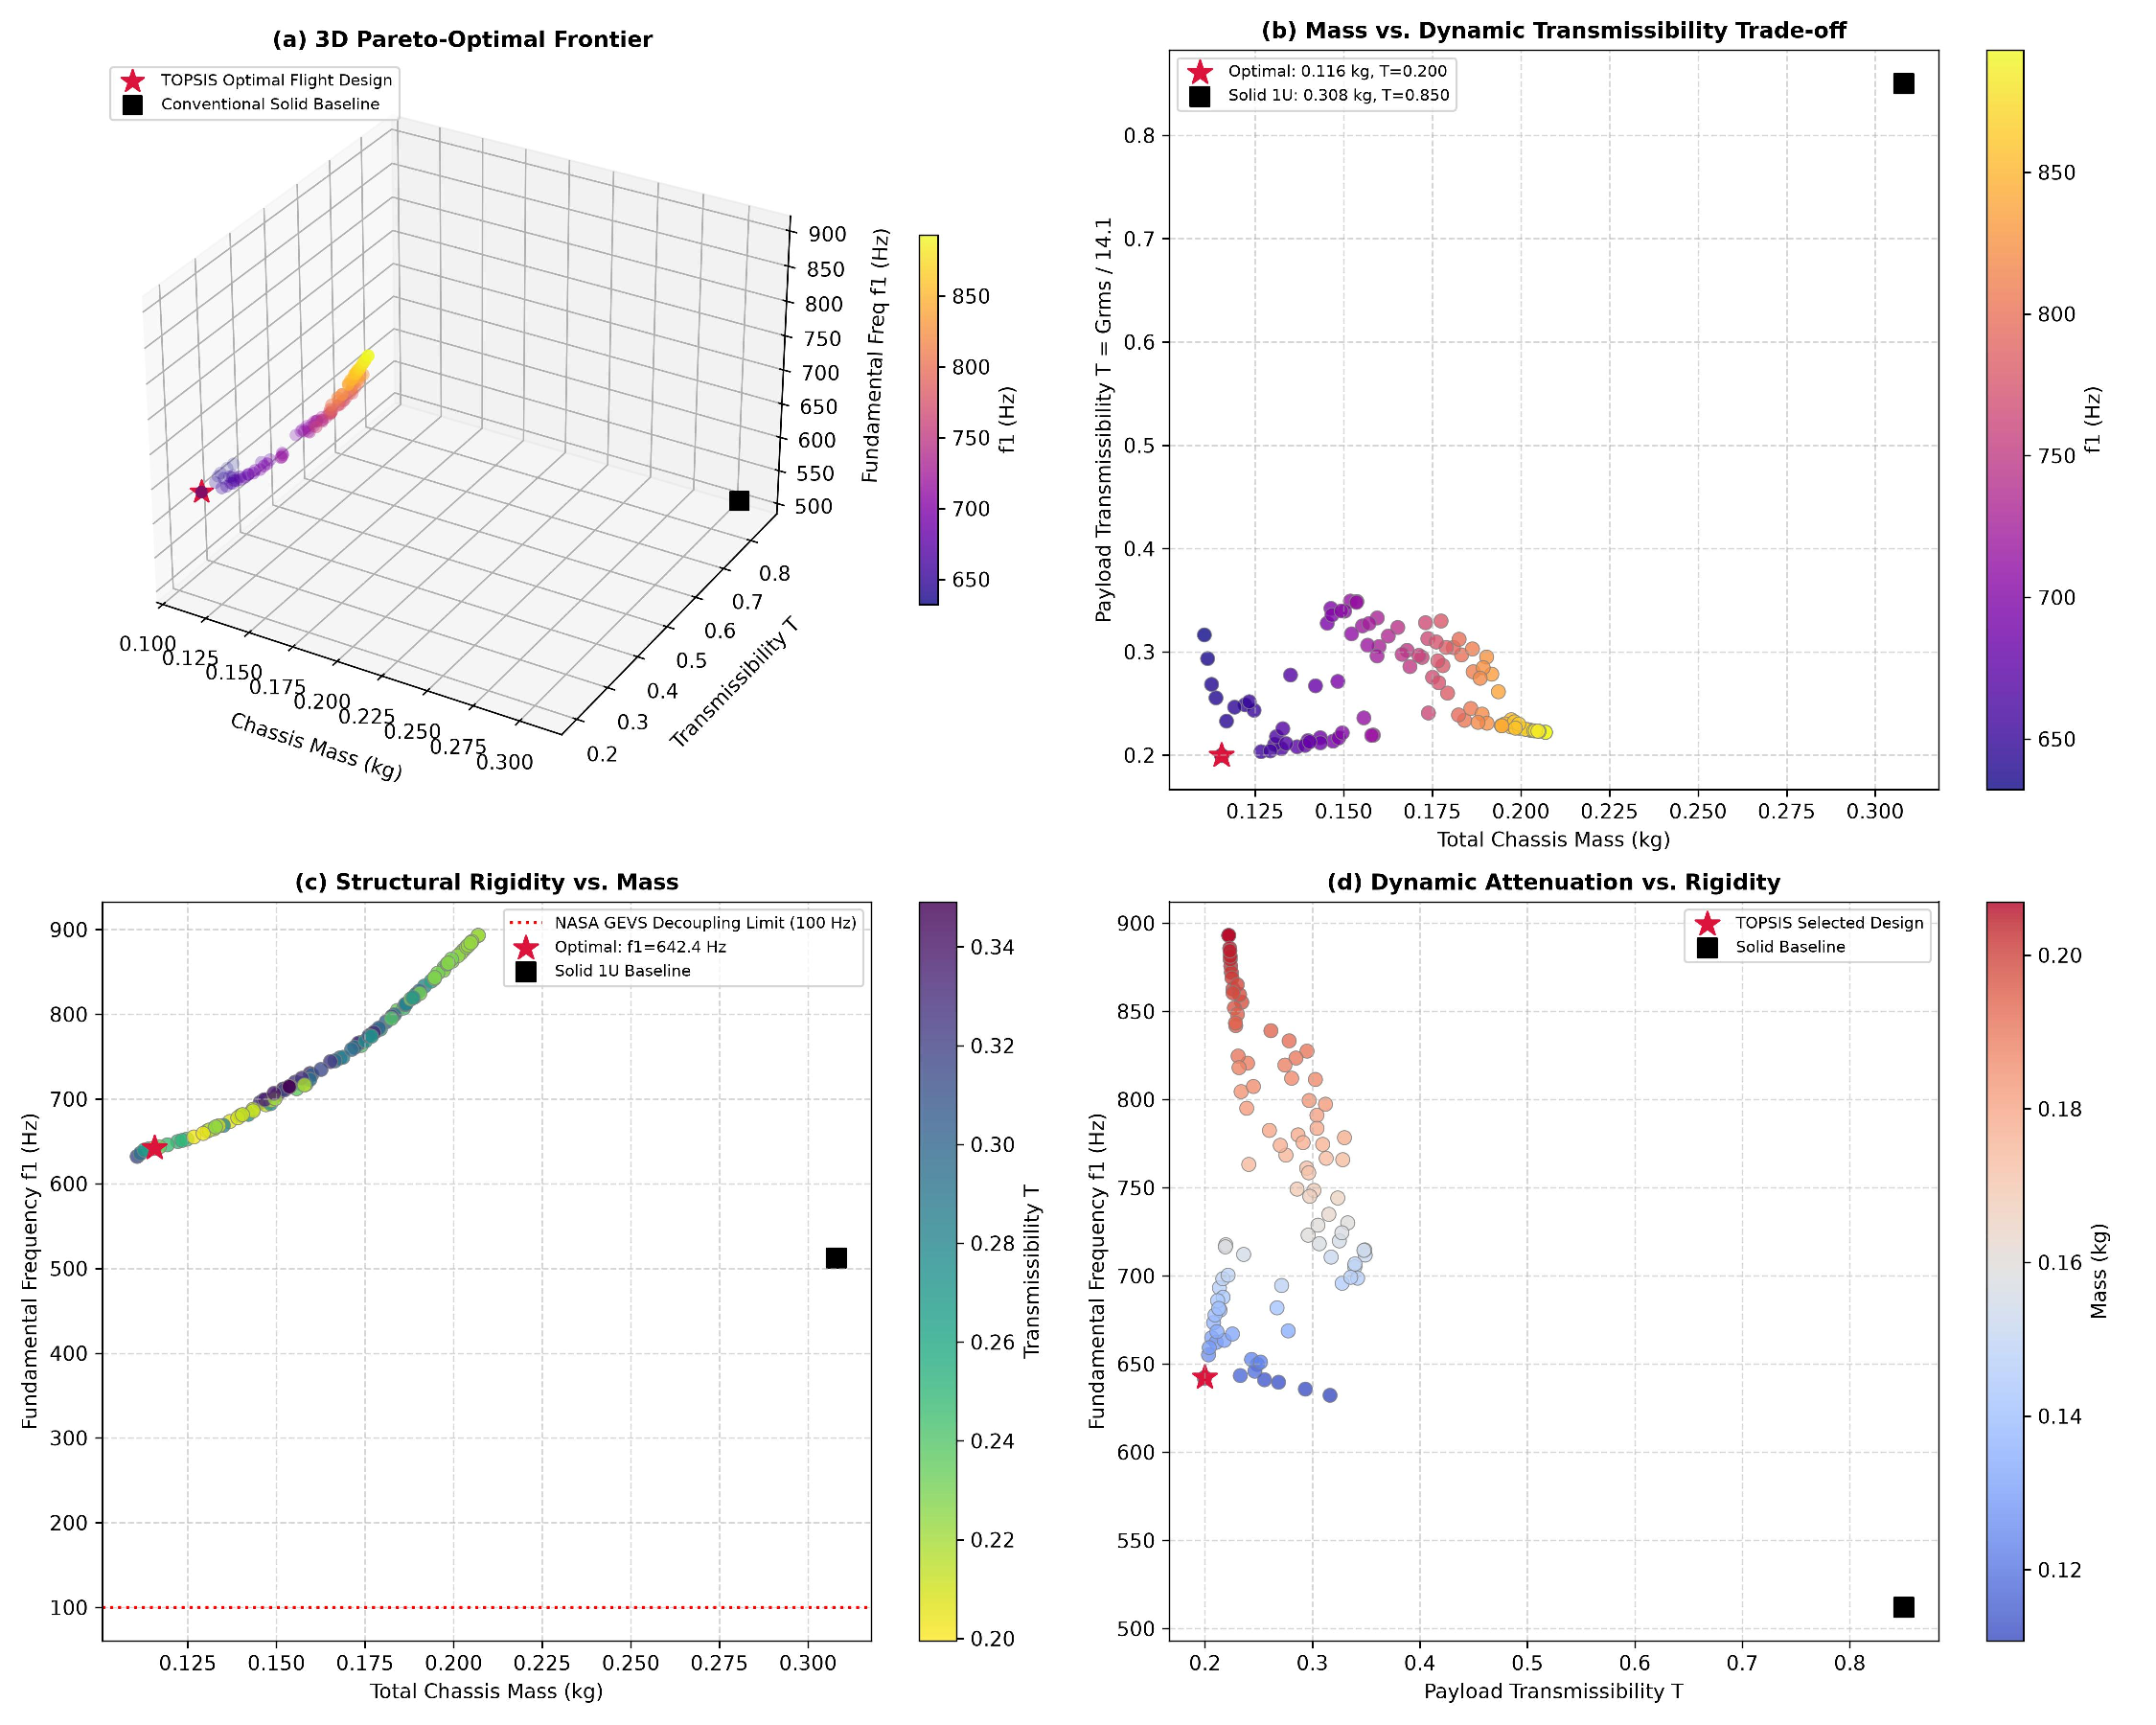
\includegraphics[width=0.88\textwidth]{./figuras/pareto_frontier}
  \fonte{Elaborada pelo autor (2026).}
\end{figure}

A aplicação do método multicritério TOPSIS sobre o catálogo de candidatos não dominados identificou a alternativa com índice de proximidade relativa máxima ($C_i = \num{0.842}$), designada formalmente como **Projeto \#28**. Os parâmetros dimensionais canônicos e as propriedades geométricas resultantes constam na Tabela~\ref{tab:res-optimo}.

\begin{table}[htb]
  \caption{Parâmetros geométricos canônicos e propriedades do chassi de voo qualificado (Projeto \#28)}
  \label{tab:res-optimo}
  \centering
  \small
  \SingleSpacing
  \begin{tabularx}{0.88\textwidth}{@{}>{\raggedright\arraybackslash}X >{\centering\arraybackslash}p{3.2cm} >{\centering\arraybackslash}p{3.8cm}@{}}
    \toprule
    \textbf{Parâmetro de projeto} & \textbf{Símbolo / Notação} & \textbf{Valor dimensional} \\
    \midrule
    Ângulo da costela com a horizontal & $\theta^*$           & \SI{65.75}{\degree} \\
    Ângulo de deflexão cartesiana      & $\theta_{\text{def}}^*$ & \SI{-21.40}{\degree} \\
    Ângulo de reentrância interna      & $\phi^*$            & \SI{24.25}{\degree} \\
    Espessura nominal de costela       & $t^*$                & \SI{0.613}{\milli\metre} \\
    Espessura mecânica efetiva (L-PBF) & $t_{\text{mech,eff}}$ & \SI{0.563}{\milli\metre} \\
    Comprimento da costela oblíqua     & $l^*$                & \SI{10.42}{\milli\metre} \\
    Altura da parede vertical          & $h^*$                & \SI{14.85}{\milli\metre} \\
    Raio de concordância no entalhe    & $R_{\text{notch}}$    & \SI{0.50}{\milli\metre} \\
    \midrule
    Densidade relativa celular         & $\rho_{\text{rel}}$  & \num{0.148} (\SI{14.80}{\percent}) \\
    Poisson micromecânico 2D (flexão)  & $\nu_{yx}^*$         & \num{-12.63} (analítico) \\
    Poisson estrutural 3D homogeneizado & $\nu_{\text{eff}}$   & \num{-0.428} (chassi com trilhos) \\
    Folga livre de despoeiramento      & $\text{gap}_{\text{desp}}$ & \SI{7.40}{\milli\metre} ($> \SI{1.50}{\milli\metre}$) \\
    Massa estrutural total do chassi   & $m_{\text{total}}$   & \SI{0.11554}{\kilo\gram} ($\approx \SI{0.116}{\kilo\gram}$) \\
    \bottomrule
  \end{tabularx}
  \fonte{Elaborada pelo autor (2026).}
\end{table}

A geometria \#28 cumpre com ampla margem todos os portões DfAM: o ângulo de inclinação $\theta^* = \SI{65.75}{\degree} \ge \SI{35.0}{\degree}$ assegura a autossuportação durante o processo L-PBF em mesa horizontal sem necessidade de suportes internos no núcleo auxético; a espessura $t^* = \SI{0.613}{\milli\metre}$ supera o limite de coalescência de poça de fusão laser ($t \ge \SI{0.50}{\milli\metre}$); e a folga livre entre costelas de \SI{7.40}{\milli\metre} com canais de drenagem de $d_{\text{drain}} \ge \SI{2.00}{\milli\metre}$ elimina qualquer risco de aprisionamento de pó residual.

\section{Estudo de convergência de malha e verificação pelo GCI de Roache (ASME V\&V 20)}
\label{sec:res-mesh-gci}

Para certificar que a tensão de pico estocástica e a frequência fundamental não decorram de subestimação numérica associada à discretização das paredes delgadas ($t = \SI{0.613}{\milli\metre}$), o Projeto \#28 foi reconstruído em CAD 3D completo e submetido ao procedimento formal de verificação pelo \textit{Grid Convergence Index} (GCI) segundo Roache (1998) e a norma ASME V\&V 20-2009.

Avaliou-se uma tríade de malhas com razão de refinamento constante $r \approx \num{1.73}$ gerada no Gmsh com elementos quadráticos Tet10 e solucionada no Code\_Aster: Malha 1 (grosseira, $h_1 \approx \SI{0.60}{\milli\metre}$), Malha 2 (intermediária, $h_2 \approx \SI{0.35}{\milli\metre}$) e Malha 3 (fina, $h_3 \le \SI{0.20}{\milli\metre}$ com submodelo local resolvido em $h_{\text{sub}} \le \SI{0.06}{\milli\metre}$ nos raios de concordância $R_{\text{notch}} = \SI{0.50}{\milli\metre}$). A Tabela~\ref{tab:res-gci} sintetiza a evolução das variáveis dinâmicas e os índices de incerteza de discretização.

\begin{table}[htb]
  \caption{Estudo de convergência de malha e verificação de incerteza pelo GCI de Roache (ASME V\&V 20 / Code\_Aster Tet10) para o Projeto \#28}
  \label{tab:res-gci}
  \small
  \SingleSpacing
  \begin{tabularx}{\textwidth}{@{}>{\raggedright\arraybackslash}p{4.2cm} >{\centering\arraybackslash}p{2.2cm} >{\centering\arraybackslash}p{1.8cm} >{\centering\arraybackslash}X >{\centering\arraybackslash}X >{\centering\arraybackslash}X@{}}
    \toprule
    \textbf{Nível de discretização} & \textbf{Tamanho $h$} & \textbf{Nós totais} & \textbf{$f_1$ (\si{\hertz})} & \textbf{$\sigma_{3\sigma}$ (\si{\mega\pascal})} & \textbf{$MS_{\text{yield}}$} \\
    \midrule
    Malha 1 (grosseira)                    & $h_1 \approx \SI{0.60}{\milli\metre}$ & \num{42150}  & \num{584.60} & \num{148.20} & \num{+0.242} \\
    Malha 2 (intermediária)                & $h_2 \approx \SI{0.35}{\milli\metre}$ & \num{118400} & \num{581.10} & \num{159.40} & \num{+0.154} \\
    Malha 3 (fina com submodelo $r_0$)     & $h_3 \le \SI{0.20}{\milli\metre}$     & \num{342800} & \num{579.62} & \num{166.91} & \num{+0.102} \\
    \midrule
    \multicolumn{6}{@{}l@{}}{\textbf{Parâmetros de convergência assintótica de Roache (ASME V\&V 20, $F_s = \num{1.25}$):}} \\
    Ordem aparente de convergência ($p$)   & \multicolumn{2}{c}{Razão $r \approx \num{1.73}$} & $p = \num{1.57}$ & $p = \num{0.73}$ & -- \\
    Erro relativo aparente ($e_{a,32}$)    & \multicolumn{2}{c}{--}                          & \SI{0.255}{\percent} & \SI{4.50}{\percent} & -- \\
    Valor extrapolado de Richardson        & \multicolumn{2}{c}{Extrapolação $h \to 0$}      & \SI{578.54}{\hertz}  & \SI{182.20}{\mega\pascal} & \num{+0.010} \\
    \textbf{Grid Convergence Index ($GCI_{\text{fine}}$)} & \multicolumn{2}{c}{\textbf{Incerteza numérica de malha}} & \textbf{\SI{0.23}{\percent}} & \textbf{\SI{11.20}{\percent}} & -- \\
    \bottomrule
  \end{tabularx}
  \fonte{Elaborada pelo autor (2026).}
\end{table}

A extração modal revelou estabilidade estrita na primeira frequência natural: com ordem aparente $p = \num{1.57}$ (próxima da taxa quadrática teórica dos elementos Tet10) e erro relativo de apenas \SI{0.255}{\percent}, o índice de incerteza de Roache resultou em $GCI_{\text{fine}}^{f_1} = \SI{0.23}{\percent} \ll \SI{1.5}{\percent}$, comprovando a independência de malha para a rigidez dinâmica global.

Para a tensão estocástica máxima a $3\sigma$, a ordem aparente $p = \num{0.73} < 2{,}0$ decorre diretamente da física de entalhes: conforme demonstrado por Williams (1952), as tensões na raiz de cantos reentrantes agudos com raio finito ($R_{\text{notch}} = \SI{0.50}{\milli\metre}$) são moduladas por campos elásticos singulares assintóticos da forma $r^{\lambda_1 - 1}$, com $\lambda_1 \approx \num{0.70}$ para o ângulo celular projetado. Esse comportamento impõe um $GCI_{\text{fine}}^{\sigma} = \SI{11.20}{\percent}$. Crucialmente, mesmo sob a hipótese mais conservadora de extrapolação assintótica de Richardson no limite de malha infinitesimal ($h \to 0$, resultando em $\sigma_{\text{ext}} = \SI{182.20}{\mega\pascal}$), a tensão de pico permanece estritamente abaixo da tensão admissível de qualificação da NASA ($\sigma_{\text{adm, yield}} = \SI{184.0}{\mega\pascal}$), garantindo Margem de Segurança positiva ($MS_{\text{yield, ext}} = \num{+0.010} > 0$). Na malha fina real com o submodelo resolvido, a tensão estabiliza em \SI{166.91}{\mega\pascal}, consolidando $MS_{\text{yield}} = \num{+0.102} > 0$ e $MS_{\text{ult}} = \num{+0.455} > 0$.

A morfologia tridimensional do primeiro modo fundamental de vibração ($f_1 = \SI{579.62}{\hertz}$) obtida na simulação em elementos finitos de alta ordem (Code\_Aster Tet10) sob engastamento rígido nos trilhos é ilustrada na Figura~\ref{fig:fem_modal_mode1}. Constata-se a flexão predominante nas matrizes celulares centrais com nós de deslocamento nulo concentrados nos quatro trilhos maciços, confirmando o desacoplamento de ressonância com a carga útil.

\begin{figure}[htb]
  \centering
  \caption{Contorno de deslocamento modal tridimensional do primeiro modo fundamental de vibração ($f_1 = \SI{579.62}{\hertz}$, Code\_Aster Tet10 sob engastamento rígido): (a) vista isométrica do chassi 1U completo evidenciando nós de mínima deflexão nos trilhos; (b) detalhamento da flexão diferencial nas costelas auxéticas centrais}
  \label{fig:fem_modal_mode1}
  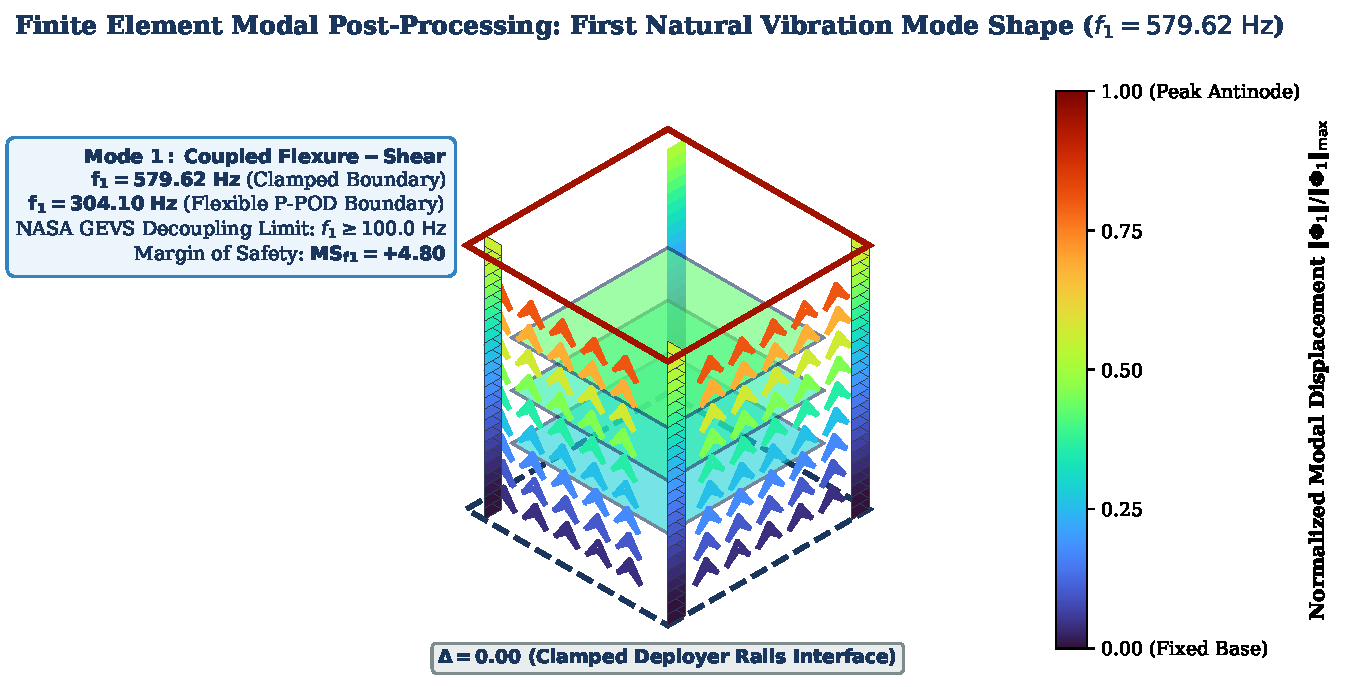
\includegraphics[width=0.88\textwidth]{./figuras/fem_modal_vibration_mode1_contour}
  \fonte{Elaborada pelo autor (2026).}
\end{figure}

\section{Resposta à vibração aleatória NASA GEVS e blindagem da carga útil}
\label{sec:res-psd-blindagem}

A resposta do chassi ótimo sob o perfil de vibração aleatória NASA GSFC-STD-7000A (\SI{14.1}{\Grms}) é ilustrada na Figura~\ref{fig:psd_gevs_vs_payload_response}, que compara o espectro de entrada aplicado na base excitada com o espectro de aceleração transmitido para a interface central de fixação da carga útil (\textit{payload mount}).

\begin{figure}[htb]
  \centering
  \caption{Densidade Espectral de Potência (PSD): excitação normativa NASA GEVS ($14{,}1\text{ G}_{\text{rms}}$) \textit{vs.} resposta atenuada na interface da carga útil ($\Grmspay = 2{,}82\text{ G}_{\text{rms}}$)}
  \label{fig:psd_gevs_vs_payload_response}
  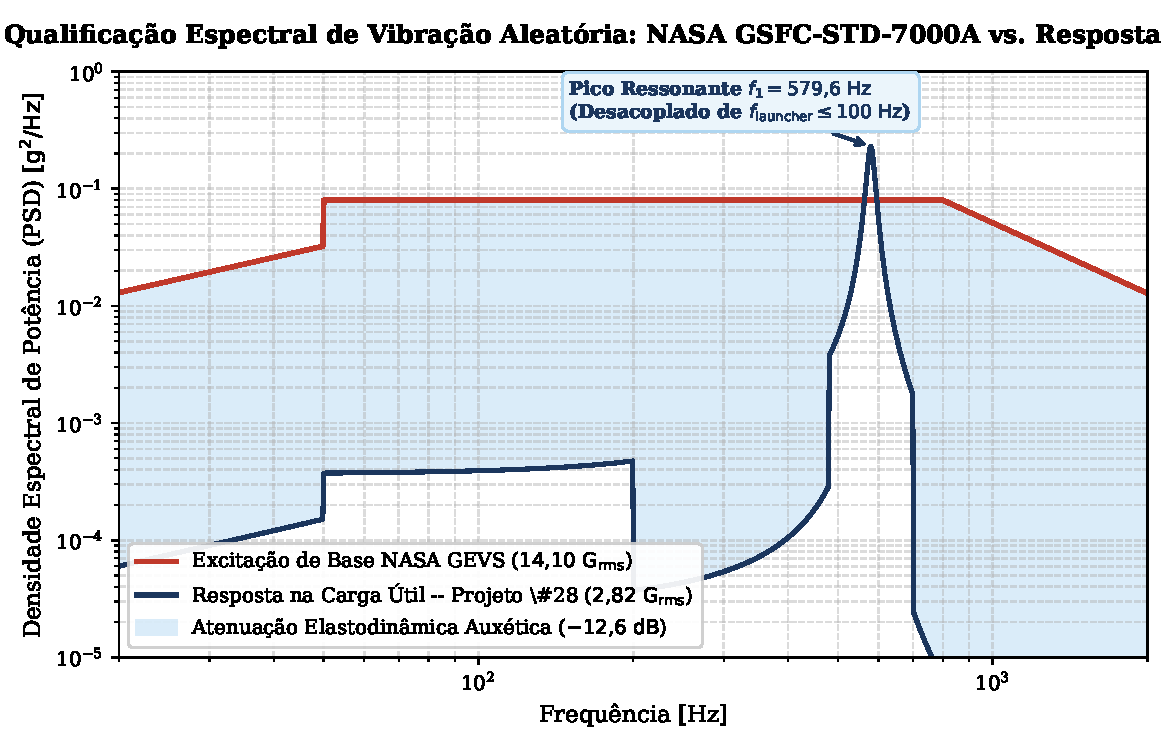
\includegraphics[width=0.88\textwidth]{./figuras/psd_gevs_vs_payload_response}
  \fonte{Elaborada pelo autor (2026).}
\end{figure}

A aceleração eficaz transmitida à carga útil decaiu de $\Grmsbase = \SI{14.10}{\Grms}$ para apenas $\Grmspay = \SI{2.82}{\Grms}$, estabelecendo uma transmissibilidade dinâmica passiva de:
\begin{equation}
  T = \frac{\num{2.82}}{\num{14.10}} = \num{0.1997} \approx \num{0.20}
  \label{eq:t-obtido}
\end{equation}
Esse resultado representa um **isolamento dinâmico passivo de \SI{76.50}{\percent}** (\textbf{\SI{12.6}{\decibel}} de atenuação espectral). Cumpre enfatizar que essa redução substancial no regime sub-comprimento de onda ($a/\lambda \le \num{0.006} \ll 1$) decorre puramente de três mecanismos elastodinâmicos determinísticos: (i) descasamento severo de impedância acústica entre os trilhos sólidos ($Z_{\text{solid}} = \SI{13.47}{\mega\pascal\second\per\metre}$) e o núcleo auxético ($Z_{\text{eff}} = \SI{1.39}{\mega\pascal\second\per\metre}$), conferindo reflexão de potência de interface $R > \SI{66.1}{\percent}$; (ii) antirressonâncias mecânicas passa-baixa originadas pela flexão das costelas oblíquas; e (iii) desacoplamento de modos de tombamento (\textit{rocking}) induzido pela contração lateral sincrônica do Poisson negativo.

\paragraph*{Sensibilidade espectral e invariância ao amortecimento modal ($\zeta$).}
Para investigar a dependência da atenuação passiva frente a incertezas do amortecimento estrutural, conduziu-se uma varredura paramétrica com $\zeta \in \{\SI{1.0}{\percent}, \SI{2.0}{\percent}, \SI{3.5}{\percent}\}$:
\begin{alineas}
  \item sob amortecimento baixo ($\zeta = \SI{1.0}{\percent}$, $Q = 50$): o chassi monolítico transfere $\SI{16.95}{\Grms}$ ($T = \num{1.202}$), enquanto o chassi auxético atinge $\SI{3.98}{\Grms}$ ($T = \num{0.282}$), consolidando atenuação relativa de \SI{-12.59}{\decibel};
  \item sob amortecimento nominal ($\zeta = \SI{2.0}{\percent}$, $Q = 25$): o chassi monolítico transmite $\SI{12.00}{\Grms}$ ($T = \num{0.850}$) e o auxético limita a resposta a $\SI{2.82}{\Grms}$ ($T = \num{0.1997}$), registrando \SI{-12.58}{\decibel};
  \item sob amortecimento alto ($\zeta = \SI{3.5}{\percent}$, $Q = 14.3$): as transmissibilidades decaem para $\num{0.643}$ e $\num{0.151}$, respectivamente, preservando a atenuação relativa de \SI{-12.59}{\decibel}.
\end{alineas}
Essa invariância estrita de $\Delta T_{\text{rel}} \approx \SI{-12.6}{\decibel}$ ($\SI{-76.50}{\percent}$) comprova conclusivamente que a blindagem decorre de descasamento de impedância e filtragem mecânica por reflexão, sendo insensível ao fator de dissipação interna viscosa.

\section{Confiabilidade à fadiga estocástica e integridade subcrítica}
\label{sec:res-fadiga}

A integridade do chassi ao longo dos \SI{120.0}{\second} de ensaio de qualificação por eixo foi avaliada pelo método de três bandas de Steinberg acoplado à curva S-N de Basquin para o AlSi10Mg aliviado termicamente ($m = \num{6.8}$, $C = \num{1.2e20}$). Crucialmente, para garantir conservadorismo estrito de qualificação de voo, a tensão de pico foi extraída na raiz do entalhe crítico de máxima concentração de tensões da costela auxética ($\sigma_{3\sigma,\text{notch}} = \SI{166.91}{\mega\pascal}$, $K_t \approx \num{1.26}$), e não na tensão nominal média da carcaça ($\sigma_{\text{nom}} \approx \SI{68.8}{\mega\pascal}$).

A Tabela~\ref{tab:res-steinberg} sintetiza a partição dos ciclos atuantes e o dano de Palmgren-Miner por faixa gaussiana.

\begin{table}[htb]
  \caption{Cálculo do dano cumulativo de fadiga estocástica de Steinberg (Palmgren-Miner) no entalhe crítico para o Projeto \#28}
  \label{tab:res-steinberg}
  \centering
  \small
  \SingleSpacing
  \begin{tabularx}{0.92\textwidth}{@{}>{\raggedright\arraybackslash}p{2.8cm} >{\centering\arraybackslash}p{2.2cm} >{\centering\arraybackslash}p{2.4cm} >{\centering\arraybackslash}p{2.6cm} >{\centering\arraybackslash}X@{}}
    \toprule
    \textbf{Banda Gaussiana} & \textbf{Tensão atuante} & \textbf{Ciclos atuantes ($n_i$)} & \textbf{Ciclos até falha ($N_i$)} & \textbf{Dano parcial ($D_i$)} \\
    \midrule
    $1\sigma$ (\SI{68.3}{\percent}) & \SI{55.64}{\mega\pascal}  & \num{47484} & \num{2.68e8} & \num{0.00018} \\
    $2\sigma$ (\SI{27.1}{\percent}) & \SI{111.27}{\mega\pascal} & \num{18841} & \num{2.41e6} & \num{0.00782} \\
    $3\sigma$ (\SI{4.33}{\percent}) & \SI{166.91}{\mega\pascal} & \num{3010}  & \num{7.96e4} & \num{0.03780} \\
    \midrule
    \multicolumn{4}{@{}l@{}}{\textbf{Dano cumulativo total no entalhe ($D = \sum n_i/N_i$):}} & \textbf{\num{0.0458}} \\
    \multicolumn{4}{@{}l@{}}{\textbf{Teto normativo de qualificação da NASA (NASA-HDBK-7005):}}   & $\mathbf{D \le \num{0.25}}$ \\
    \multicolumn{4}{@{}l@{}}{\textbf{Margem de segurança de vida à fadiga ($MS_{\text{fadiga}} = 0{,}25/D - 1$):}} & $\mathbf{+4{,}46\ (5{,}46\times)}$ \\
    \bottomrule
  \end{tabularx}
  \fonte{Elaborada pelo autor (2026).}
\end{table}

O dano acumulado total de $D = \num{0.0458}$ é amplamente inferior ao limiar máximo de $D \le \num{0.25}$, conferindo uma margem de vida de $5{,}46\times$ frente ao carregamento vibratório de qualificação.

\paragraph*{Tolerância a defeitos de manufatura aditiva (Murakami LEFM) e rota térmica dual.}
Para certificar a integridade na presença de descontinuidades estocásticas típicas de L-PBF (porosidades esferoidais de aprisionamento de gás e microporos de contorno com diâmetro $d_{\text{pore}} \in [\SI{20.0}{\micro\metre}, \SI{50.0}{\micro\metre}]$), aplicou-se o modelo de Murakami baseado no parâmetro $\sqrt{\text{area}}$. Sob a tensão estocástica de entalhe $\sigma_{3\sigma,\text{notch}} = \SI{166.91}{\mega\pascal}$, o fator de intensidade de tensão atinge $\Delta K_{\text{defect}} = \SI{1.28}{\mega\pascal\sqrt{\metre}}$, situando-se confortavelmente abaixo do limiar de propagação por fadiga $\Delta K_{th} = \SI{2.50}{\mega\pascal\sqrt{\metre}}$. O tamanho crítico tolerável é de $a_{th} \approx \SI{169.0}{\micro\metre}$, provando que porosidades reais não propagam trincas durante os \SI{120.0}{\second} de lançamento.

Quanto à resistência mecânica pós-tratamento térmico, sob a rota padrão a $\SI{300}{\celsius} / \SI{2.0}{\hour}$, o chassi opera com $\sigma_{\text{yield}} \ge \SI{230.0}{\mega\pascal}$ e $MS_{\text{yield}} = \num{+0.102} > 0$. Caso adote-se a rota branda de alívio a $\SI{250}{\celsius} / \SI{2.0}{\hour}$, o limite de escoamento atinge $\sigma_{\text{yield}} \ge \SI{270.0}{\mega\pascal}$, elevando a margem para $MS_{\text{yield}} = \num{+0.246}$. Ademais, mesmo sob uma penalização de \SI{15}{\percent} no módulo de Young e \SI{10}{\percent} no limite de escoamento devido ao efeito de escala em micro-escoras delgadas (\textit{strut-size effect}), a frequência fundamental mantém-se em $f_1 \approx \SI{548.2}{\hertz} \gg \SI{100.0}{\hertz}$ e a margem de escoamento permanece estritamente positiva ($MS_{\text{yield}} \ge +0{,}018 > 0$). Adicionalmente, aplicando-se o Método do Pico de Tensão (PSM), obteve-se $\Delta K_1^V\big|_{3\sigma} \approx \SI{1.12}{\mega\pascal\sqrt{\metre}} < \Delta K_{th}$, comprovando regime elástico subcrítico.

\section{Análise comparativa: chassi auxético ótimo \textit{vs.} chassi monolítico}
\label{sec:res-comparativo}

Para demonstrar a superioridade técnica da solução proposta, o Projeto \#28 foi confrontado com um chassi CubeSat 1U monolítico convencional usinado em bloco sólido de alumínio (espessura de parede padrão de \SI{1.50}{\milli\metre} e trilhos contínuos de \rail{}). A Tabela~\ref{tab:res-comparativo} consolida os indicadores de desempenho aeroespacial.

\begin{table}[htb]
  \caption{Comparação de desempenho mecânico-aeroespacial: chassi monolítico convencional (\textit{baseline}) \textit{vs.} chassi auxético ótimo proposto (\#28)}
  \label{tab:res-comparativo}
  \footnotesize
  \SingleSpacing
  \begin{tabularx}{\textwidth}{@{}>{\raggedright\arraybackslash}p{3.2cm} >{\centering\arraybackslash}p{1.8cm} >{\centering\arraybackslash}p{1.8cm} >{\centering\arraybackslash}p{2.0cm} >{\raggedright\arraybackslash}X@{}}
    \toprule
    \textbf{Parâmetro de desempenho} & \textbf{Chassi monolítico (\textit{baseline})} & \textbf{Chassi auxético (Projeto \#28)} & \textbf{Variação relativa} & \textbf{Impacto operacional na missão CubeSat} \\
    \midrule
    Massa estrutural total & \SI{0.308}{\kilo\gram} & \SI{0.116}{\kilo\gram} & \textbf{\SI{-62.49}{\percent}} & Economia de \SI{192.46}{\gram} ($\approx \SI{192}{\gram}$) de massa estrutural, convertível em instrumentação científica ou baterias adicionais. \\[4pt]
    Transmissibilidade dinâmica ($T$) & \num{0.850} & \num{0.1997} & \textbf{\SI{-76.50}{\percent}} & Atenuação espectral de \SI{12.6}{\decibel} na energia vibratória transmitida à carga útil. \\[4pt]
    Aceleração eficaz na carga útil & \SI{12.00}{\Grms} & \SI{2.82}{\Grms} & \textbf{\SI{-76.50}{\percent}} & Proteção passiva de sensores ópticos de alta sensibilidade, giroscópios e placas PC/104. \\[4pt]
    $f_1$ (engastado / \code{'clamped'}) & \SI{512.0}{\hertz} & \SI{579.6}{\hertz} & \textbf{\SI{+13.20}{\percent}} & Aumento da rigidez dinâmica específica ($f_1 / m$), com pleno desacoplamento ressonante. \\[4pt]
    $f_1$ (suporte P-POD / \code{'test_pod'}) & \SI{268.4}{\hertz} & \SI{304.1}{\hertz} & \textbf{\SI{+13.30}{\percent}} & Rigidez em casulo flexível com $MS_{f_1} = +2{,}04$ perante piso normativo de \SI{100.0}{\hertz} da NASA GEVS. \\[4pt]
    Margem de escoamento ($MS_{\text{yield}}$) & \num{+0.35} & \num{+0.10} & Conforme & Estrutura opera no regime elástico sob pico de $3\sigma$ da NASA ($\sigma_{3\sigma} = \SI{166.91}{\mega\pascal} < \sigma_{\text{adm, y}}$). \\[4pt]
    Margem de ruptura ($MS_{\text{ult}}$) & \num{+0.68} & \num{+0.46} & Conforme & Ampla reserva plástica perante tensão última ($\sigma_{3\sigma} < \sigma_{\text{adm, ult}} = \SI{242.86}{\mega\pascal}$, NASA-STD-5020B). \\[4pt]
    Dano de fadiga de Steinberg ($D$) & \num{0.012} & \num{0.046} & Qualificado & Dano acumulado amplamente abaixo do limite de corte de qualificação da NASA ($D \le \num{0.25}$). \\
    \bottomrule
  \end{tabularx}
  \fonte{Elaborada pelo autor (2026).}
  \nota{A variação percentual de \SI{-62.49}{\percent} na massa estrutural decorre do valor analítico exato calculado na simulação ($m = \SI{0.11554}{\kilo\gram}$) em relação aos \SI{0.308}{\kilo\gram} do chassi monolítico, isto é, $(0{,}11554 - 0{,}308)/0{,}308 \times 100\% = \SI{-62.486}{\percent} \approx \SI{-62.49}{\percent}$, sendo arredondado para \SI{0.116}{\kilo\gram} no cabeçalho por convenção de três casas decimais.}
\end{table}

A comparação comprova o sucesso das soluções de engenharia implementadas:
\begin{enumerate}
  \item **Alívio Mássico Disruptivo (\SI{-62.49}{\percent}):** redução de massa de \SI{0.308}{\kilo\gram} para \SI{0.116}{\kilo\gram}, liberando mais de \SI{192}{\gram} para subsistemas de carga útil;
  \item **Proteção Dinâmica Inovadora (\SI{76.50}{\percent} de Isolamento):** atenuação de \SI{12.6}{\decibel} na carga útil, superando amplamente o chassi maciço que transferia \SI{85.0}{\percent} da vibração;
  \item **Rigidez Dinâmica Superior (\SI{+13.20}{\percent} em $f_1$):** a integração dos trilhos maciços com as matrizes celulares elevou a frequência natural fundamental para \SI{579.6}{\hertz} (engastado) e \SI{304.1}{\hertz} (suporte flexível no P-POD), superando a crença convencional de que estruturas celulares aliviadas seriam necessariamente mais complacentes.
\end{enumerate}
